\documentclass{article}
\usepackage[T1]{fontenc}
\usepackage{lmodern}
\usepackage{graphicx}
\usepackage{amsmath,amssymb}
\usepackage[a4paper,margin=2cm]{geometry}
\usepackage[absolute,overlay]{textpos}
\setlength{\TPHorizModule}{1mm}
\setlength{\TPVertModule}{1mm}
\usepackage[indonesian]{babel}
\usepackage{hyperref}
\setlength{\emergencystretch}{2em}
% unit: Halaman 27

\begin{document}

% === Halaman 27 (python/native) ===

Jika diteruskan untuk x = 4, 5, …, 10, diperoleh tabel sebagai berikut :

27

Jadi, titik-titik yang terdapat pada

kurva eliptik adalah 12, yaitu:

(2, 4), (2, 7), (3, 5), (3, 6), (5, 2),

(5, 9), (7, 2), (7, 9), (8, 3), (8, 8),

(10, 2), (10, 9)

Jika ditambah dengan titik O di 

infinity, maka titik-titik pada 

kurva eliptik membentuk grup

dengan n = 13 elemen.

Sumber: Andreas Steffen, 

Elliptic Curve Cryptography

% deskripsi: gambar native xref 119
\noindent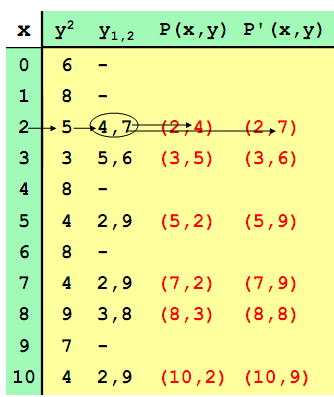
\includegraphics[width=0.85\textwidth]{../../images/python/page_027_img_01.png}

\end{document}
